\documentclass[11pt,preprint, authoryear]{elsarticle}

\usepackage{lmodern}
%%%% My spacing
\usepackage{setspace}
\setstretch{1.2}
\DeclareMathSizes{12}{14}{10}{10}

% Wrap around which gives all figures included the [H] command, or places it "here". This can be tedious to code in Rmarkdown.
\usepackage{float}
\let\origfigure\figure
\let\endorigfigure\endfigure
\renewenvironment{figure}[1][2] {
    \expandafter\origfigure\expandafter[H]
} {
    \endorigfigure
}

\let\origtable\table
\let\endorigtable\endtable
\renewenvironment{table}[1][2] {
    \expandafter\origtable\expandafter[H]
} {
    \endorigtable
}


\usepackage{ifxetex,ifluatex}
\usepackage{fixltx2e} % provides \textsubscript
\ifnum 0\ifxetex 1\fi\ifluatex 1\fi=0 % if pdftex
  \usepackage[T1]{fontenc}
  \usepackage[utf8]{inputenc}
\else % if luatex or xelatex
  \ifxetex
    \usepackage{mathspec}
    \usepackage{xltxtra,xunicode}
  \else
    \usepackage{fontspec}
  \fi
  \defaultfontfeatures{Mapping=tex-text,Scale=MatchLowercase}
  \newcommand{\euro}{€}
\fi

\usepackage{amssymb, amsmath, amsthm, amsfonts}

\def\bibsection{\section*{References}} %%% Make "References" appear before bibliography


\usepackage[round]{natbib}

\usepackage{longtable}
\usepackage[margin=2.3cm,bottom=2cm,top=2.5cm, includefoot]{geometry}
\usepackage{fancyhdr}
\usepackage[bottom, hang, flushmargin]{footmisc}
\usepackage{graphicx}
\numberwithin{equation}{section}
\numberwithin{figure}{section}
\numberwithin{table}{section}
\setlength{\parindent}{0cm}
\setlength{\parskip}{1.3ex plus 0.5ex minus 0.3ex}
\usepackage{textcomp}
\renewcommand{\headrulewidth}{0.2pt}
\renewcommand{\footrulewidth}{0.3pt}

\usepackage{array}
\newcolumntype{x}[1]{>{\centering\arraybackslash\hspace{0pt}}p{#1}}

%%%%  Remove the "preprint submitted to" part. Don't worry about this either, it just looks better without it:
\makeatletter
\def\ps@pprintTitle{%
  \let\@oddhead\@empty
  \let\@evenhead\@empty
  \let\@oddfoot\@empty
  \let\@evenfoot\@oddfoot
}
\makeatother

 \def\tightlist{} % This allows for subbullets!

\usepackage{hyperref}
\hypersetup{breaklinks=true,
            bookmarks=true,
            colorlinks=true,
            citecolor=blue,
            urlcolor=blue,
            linkcolor=blue,
            pdfborder={0 0 0}}


% The following packages allow huxtable to work:
\usepackage{siunitx}
\usepackage{multirow}
\usepackage{hhline}
\usepackage{calc}
\usepackage{tabularx}
\usepackage{booktabs}
\usepackage{caption}


\newenvironment{columns}[1][]{}{}

\newenvironment{column}[1]{\begin{minipage}{#1}\ignorespaces}{%
\end{minipage}
\ifhmode\unskip\fi
\aftergroup\useignorespacesandallpars}

\def\useignorespacesandallpars#1\ignorespaces\fi{%
#1\fi\ignorespacesandallpars}

\makeatletter
\def\ignorespacesandallpars{%
  \@ifnextchar\par
    {\expandafter\ignorespacesandallpars\@gobble}%
    {}%
}
\makeatother

\newlength{\cslhangindent}
\setlength{\cslhangindent}{1.5em}
\newenvironment{CSLReferences}%
  {\setlength{\parindent}{0pt}%
  \everypar{\setlength{\hangindent}{\cslhangindent}}\ignorespaces}%
  {\par}


\urlstyle{same}  % don't use monospace font for urls
\setlength{\parindent}{0pt}
\setlength{\parskip}{6pt plus 2pt minus 1pt}
\setlength{\emergencystretch}{3em}  % prevent overfull lines
\setcounter{secnumdepth}{5}

%%% Use protect on footnotes to avoid problems with footnotes in titles
\let\rmarkdownfootnote\footnote%
\def\footnote{\protect\rmarkdownfootnote}
\IfFileExists{upquote.sty}{\usepackage{upquote}}{}

%%% Include extra packages specified by user
\usepackage{booktabs}
\usepackage{longtable}
\usepackage{array}
\usepackage{multirow}
\usepackage{wrapfig}
\usepackage{float}
\usepackage{colortbl}
\usepackage{pdflscape}
\usepackage{tabu}
\usepackage{threeparttable}
\usepackage{threeparttablex}
\usepackage[normalem]{ulem}
\usepackage{makecell}
\usepackage{xcolor}

%%% Hard setting column skips for reports - this ensures greater consistency and control over the length settings in the document.
%% page layout
%% paragraphs
\setlength{\baselineskip}{12pt plus 0pt minus 0pt}
\setlength{\parskip}{12pt plus 0pt minus 0pt}
\setlength{\parindent}{0pt plus 0pt minus 0pt}
%% floats
\setlength{\floatsep}{12pt plus 0 pt minus 0pt}
\setlength{\textfloatsep}{20pt plus 0pt minus 0pt}
\setlength{\intextsep}{14pt plus 0pt minus 0pt}
\setlength{\dbltextfloatsep}{20pt plus 0pt minus 0pt}
\setlength{\dblfloatsep}{14pt plus 0pt minus 0pt}
%% maths
\setlength{\abovedisplayskip}{12pt plus 0pt minus 0pt}
\setlength{\belowdisplayskip}{12pt plus 0pt minus 0pt}
%% lists
\setlength{\topsep}{10pt plus 0pt minus 0pt}
\setlength{\partopsep}{3pt plus 0pt minus 0pt}
\setlength{\itemsep}{5pt plus 0pt minus 0pt}
\setlength{\labelsep}{8mm plus 0mm minus 0mm}
\setlength{\parsep}{\the\parskip}
\setlength{\listparindent}{\the\parindent}
%% verbatim
\setlength{\fboxsep}{5pt plus 0pt minus 0pt}



\begin{document}



\begin{frontmatter}  %

\title{Comparing Different Machine Learning Techniques for Stock Market
Predictions.}

% Set to FALSE if wanting to remove title (for submission)




\author[Add1]{Tian Cater\footnote{\textbf{Code and data:} \newline The
  code and data used in this project is readily available at
  \url{https://github.com/TianCater/Data_Science_871_Machine_Learning}.
  I would also like to thank Katzke
  (\protect\hyperlink{ref-Texevier}{2017}) for this seamless integration
  of Latex in R.}}
\ead{19025831@sun.ac.za}





\address[Add1]{Data Science 871: Machine Learning Project}



\vspace{1cm}





\vspace{0.5cm}

\end{frontmatter}



%________________________
% Header and Footers
%%%%%%%%%%%%%%%%%%%%%%%%%%%%%%%%%
\pagestyle{fancy}
\chead{}
\rhead{}
\lfoot{}
\rfoot{\footnotesize Page \thepage}
\lhead{}
%\rfoot{\footnotesize Page \thepage } % "e.g. Page 2"
\cfoot{}

%\setlength\headheight{30pt}
%%%%%%%%%%%%%%%%%%%%%%%%%%%%%%%%%
%________________________

\headsep 35pt % So that header does not go over title




\hypertarget{introduction}{%
\section{\texorpdfstring{Introduction
\label{Introduction}}{Introduction }}\label{introduction}}

Predicting future outcomes based on historical data is known as a
forecasting algorithm. Accordingly, this project implements Facebook's
Prophet, the K-Nearest Neighbours (KNN), and the Feed-forward Neural
Network (FNN) algorithms to predict the movement in value of the
Johannesburg Stock Exchange's (JSE) Top 40 Index. Importantly, these
predictions are not aimed at analysing stock price movements to provide
investor insights. Instead, the purpose is to show the models fitted,
compare the different forecasting approaches, and encourage their use.

Since the outset of financial markets, investor's have been attempting
to predict market trends and random behaviour. However, as indicated by
some of the most formidable market investors, predicting stock market
returns is almost impossible. However, all improving techniques
surrounding machine learning and its implications for forecasting time
series might someday provide more robust stock market predictions. It is
in investigating some of these machine learning techniques that give
inclination to this project.

All the models performed very well inside the prediction intervals and
the accuracy metrics, with the FNN algorithm displaying the most
accurate predictions. The KNN model did not serve as well as the Prophet
and FNN models under our metrics. This could be because KNN may need
more tuning phases, training, and testing approaches, or they are not as
effective as the other models because they mainly use classificatory
terms more than forecasting.

\hypertarget{forecasting-using-the-prophet-algorithm}{%
\section{Forecasting using the Prophet
Algorithm}\label{forecasting-using-the-prophet-algorithm}}

The Prophet model is an additive regression model developed by Taylor \&
Letham (\protect\hyperlink{ref-taylor2018}{2018}) at Facebook's Core
Data Science team, providing an effective solution to forecast time
series with trending and seasonal properties. The model consists of four
main components: A logistic growth curve or piecewise linear trend
(\(g(t)\)), a yearly seasonal element using a Fourier series (\(s(t)\)),
a weekly seasonal part using dummy variables, and the effects of
holidays or significant events (\(h(t)\)).

\begin{figure}[H]

{\centering 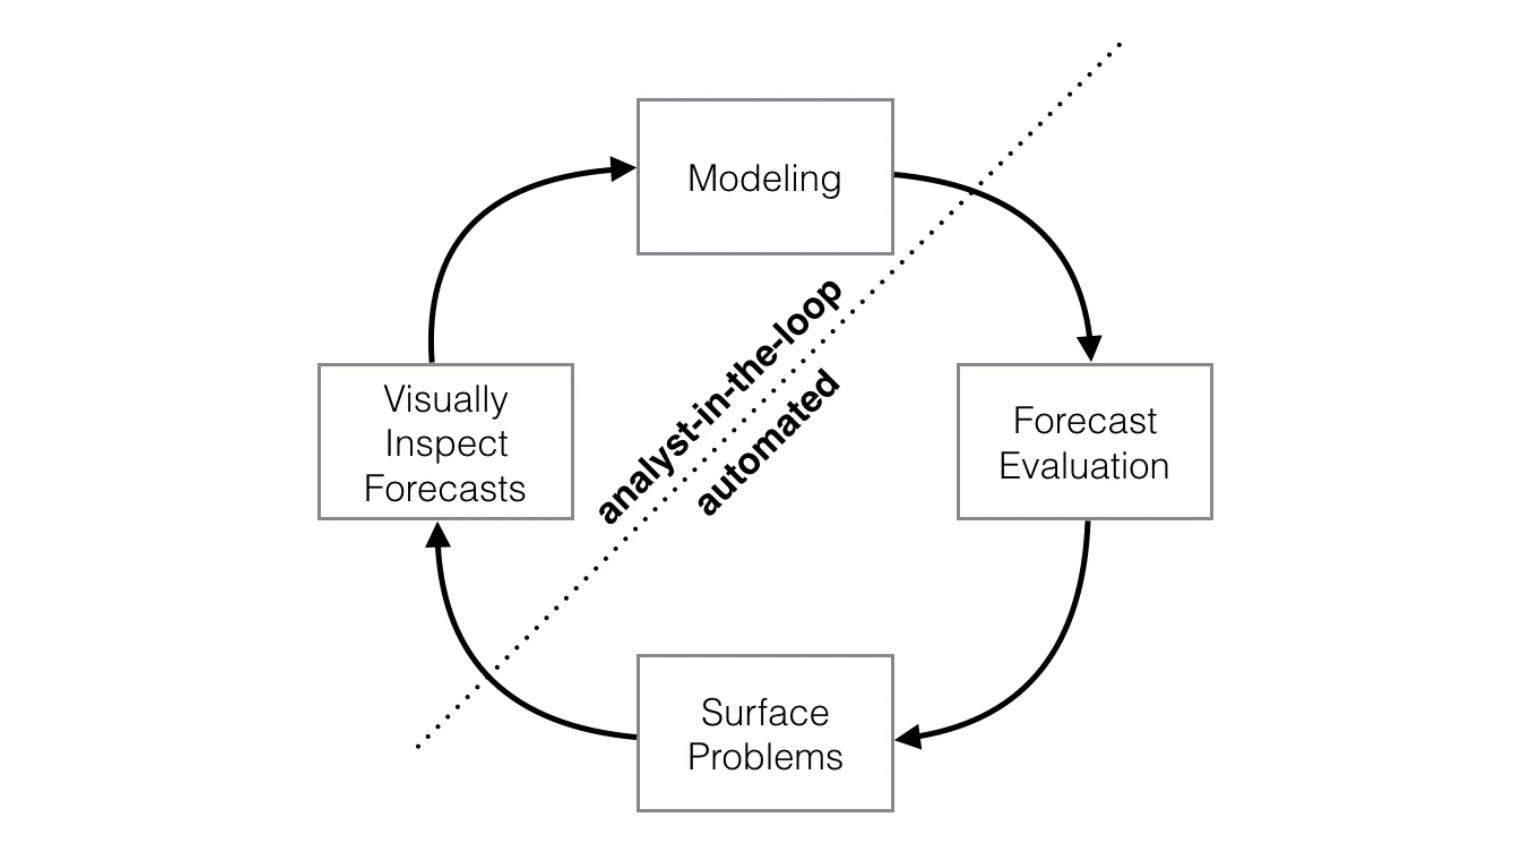
\includegraphics[width=0.7\linewidth]{code/prophet} 

}

\caption{The dynamics of the Prophet algorithm. \label{image1}}\label{fig:unnamed-chunk-1}
\end{figure}

Figure \ref{Prophet} compares the actual data versus the predicted
values fitted using a piecewise linear trend and forecasting 500
observations in advance. Additionally, the number of lags are selected
based on the Akeike Information Criteria (AIC). Visually, the predicted
values seem to do the actual data rather well. However, to better
understand the data generating process, the expected prophet components
divided by a trend component, weekly seasonality and yearly seasonality
are depicted in figure \ref{ProphetT}. Outside of the apparent weekly
seasonality due to markets being closed on weekends, the predicted
values show higher volatility during the year's first quarter. This
evidence makes sense as most companies in the JSE Top 40 index have
their financial year-end during this period.

\begin{figure}[H]

{\centering \includegraphics{JSE_Top40_Predictions_Using_Machine_Learning_files/figure-latex/unnamed-chunk-2-1} 

}

\caption{Visualisation of Train Prediction (blue) vs Observed Data (black).\label{Prophet}}\label{fig:unnamed-chunk-2}
\end{figure}

\begin{figure}[H]

{\centering \includegraphics{JSE_Top40_Predictions_Using_Machine_Learning_files/figure-latex/unnamed-chunk-3-1} 

}

\caption{Cross validation of Prophet components controlling for trend, weekly seasonality, and yearly seasonality.\label{ProphetT}}\label{fig:unnamed-chunk-3}
\end{figure}

The corresponding statistics reflecting the accuracy of the prediction
are provided in table \ref{Propheta}. All of the goodness-of-fit
statistics report that the Prophet predicted values are sufficiently
accurate in predicting the actual observations. For ease of
interpretation we consider the Mean Absolute Percentage Error (MAPE) of
4.631\%, indicating that the actual and predicted value are off by
4.63\%.\footnote{The formula for the MAPE is given by:
  \((1/n) \sum_{t=1}^T|\frac{actual \ value-predicted \ value}{actual \ value}| \times 100.\)}

\begin{table}

\caption{\label{tab:unnamed-chunk-4}Goodness of fit statistics reflecting the accuracy of the Prophet model forecasts. \label{Propheta}}
\centering
\begin{tabu} to \linewidth {>{\raggedright}X>{\centering}X>{\centering}X>{\centering}X>{\centering}X>{\centering}X}
\toprule
  & ME & RMSE & MAE & MPE & MAPE\\
\midrule
Test set & 0.015 & 234.43 & 156.524 & -0.365 & 4.361\\
\bottomrule
\end{tabu}
\end{table}

\hypertarget{the-k-nearest-neighbours-knn-algorithm}{%
\section{The K-Nearest Neighbours (KNN)
Algorithm}\label{the-k-nearest-neighbours-knn-algorithm}}

The K-Nearest Neighbours (KNN) algorithm is a supervised machine
learning algorithm first introduced by Keller, Gray \& Givens
(\protect\hyperlink{ref-keller1985}{1985}). The algorithm applies a
method of classifying data to estimate the likelihood that a data point
will become a member of one group or another depending on the group to
which the data points nearest to it belong (the training set). In this
section, our primary objective is to forecast values for the JSE Top 40
index through a KNN experimental approach and compare its forecast
accuracy with the other models adopted.

The following 500 values forecasted are shown in figure \ref{KNN}. The
number of parameters in the KNN regression is set to 100 because this
project focuses on comparing different projection models rather than
deducing the actual movement of stock prices. Furthermore, the lags are
selected based on the AIC, and recursive methods are applied as the
multiple-step ahead strategy.\footnote{See Taunk, De, Verma \&
  Swetapadma (\protect\hyperlink{ref-taunk2019}{2019}) for a detailed
  description of the intricacies surrounding the KNN algorithm.}

\begin{figure}[H]

{\centering \includegraphics{JSE_Top40_Predictions_Using_Machine_Learning_files/figure-latex/unnamed-chunk-5-1} 

}

\caption{Forecasted JSE Top 40 index using the k-nearest neigbours algorithm.\label{KNN}}\label{fig:unnamed-chunk-5}
\end{figure}

The forecasts depicted in figure \ref{KNN} indicate that the JSE Top 40
index will experience growth, with a marginally slight decline after two
months that recovers rather quickly towards its stable growth path. The
statistics that measure the accuracy of the prediction are given in
table \ref{KNNa} below. Again, referring to the MAPE value of 6.95\%,
the projections fit the actual data sufficiently, with a 6.95\% error
between the predicted and actual values. However, this is a slightly
worse fit than the predictions computed using the Prophet algorithm.

\begin{table}

\caption{\label{tab:unnamed-chunk-6}Goodness of fit statistics reflecting the accuracy of the KNN algorithms forecasts. \label{KNNa}}
\centering
\begin{tabu} to \linewidth {>{\raggedright}X>{\centering}X}
\toprule
  & x\\
\midrule
RMSE & 662.689\\
MAE & 481.607\\
MAPE & 6.947\\
\bottomrule
\end{tabu}
\end{table}

\hypertarget{the-feed-forward-neural-network-fnn}{%
\section{The Feed-forward Neural Network
(FNN)}\label{the-feed-forward-neural-network-fnn}}

\begin{figure}[H]

{\centering 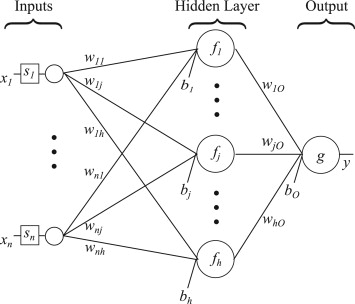
\includegraphics[width=0.55\linewidth]{code/feed_forward} 

}

\caption{The dynamics of the feed-forward neural network algorithm. \label{image2}}\label{fig:unnamed-chunk-7}
\end{figure}

A single hidden layer feed-forward neural network (FNN) is the first and
most straightforward kind of artificial neural network where connections
between nodes do not form a loop or cycle
(\protect\hyperlink{ref-sanger1989}{Sanger, 1989}). Consequently, the
information only flows forward from the input nodes through the hidden
nodes and to the output nodes. In its form considered here, only one
layer of input nodes transmits weighted inputs to the next layer of
receiving nodes.

This section fits a single hidden layer FNN to the JSE Top 40 time
series. Similar to the approach by Wang, Er \& Han
(\protect\hyperlink{ref-wang2014}{2014}), the functional model involves
using lagged values of the process as the input data, resulting in an
estimated non-linear autoregressive model.

The specific number of hidden nodes is half the number of input nodes,
including external independent variables, plus one. To ensure that the
residuals will be approximately homoscedastic, the Box-Cox lambda
approach is used. In figure \ref{FNN}, the following 500 values are
forecasted with the neural net fitted and the number of lags selected
based on the AIC. In contrast to the Prophet and KNN predictions, figure
\ref{FNN} predicts that the JSE Top 40 index will experience a sharp
decline until levelling off approximately three months later.

\begin{figure}[H]

{\centering \includegraphics{JSE_Top40_Predictions_Using_Machine_Learning_files/figure-latex/unnamed-chunk-8-1} 

}

\caption{Forecasted JSE Top 40 index using the feed-forward neural network.\label{FNN}}\label{fig:unnamed-chunk-8}
\end{figure}

The accuracy statistics are given in table \ref{FNNa} below. The MAPE of
0.95 is an improvement on both the Prophet and KNN predictions,
indicating that the actual and forecasted values are off by 0.95\%.

\begin{table}

\caption{\label{tab:Accuracy of FNN Forecast}Goodness of fit statistics reflecting the accuracy of the FNN algorithms forecasts. \label{FNNa}}
\centering
\begin{tabu} to \linewidth {>{\raggedright}X>{\centering}X>{\centering}X>{\centering}X>{\centering}X>{\centering}X>{\centering}X>{\centering}X}
\toprule
  & ME & RMSE & MAE & MPE & MAPE & MASE & ACF1\\
\midrule
Training set & 1.414 & 54.976 & 36.298 & -0.006 & 0.991 & 1.042 & 0.039\\
\bottomrule
\end{tabu}
\end{table}

\hypertarget{conclusion}{%
\section{Conclusion}\label{conclusion}}

This study focused on applying different models, learning how to use
them to forecast JSE Top 40 index values, and showcasing contrasting
results. The Prophet and KNN algorithms predicted a price increase over
the next 500 days, whereas the FNN algorithm a price decrease.

All the models performed very well inside the prediction intervals and
the accuracy metrics, with the FNN algorithm displaying the most
accurate predictions. The KNN model did not serve as well as the Prophet
and FNN models under our metrics. This could be because KNN may need
more tuning phases, training, and testing approaches, or they are not as
effective as the other models because they mainly use classificatory
terms more than forecasting.

\newpage

\hypertarget{references}{%
\section*{References}\label{references}}
\addcontentsline{toc}{section}{References}

\hypertarget{refs}{}
\begin{CSLReferences}{1}{0}
\leavevmode\vadjust pre{\hypertarget{ref-Texevier}{}}%
Katzke, N.F. 2017. \emph{{Texevier}: {P}ackage to create elsevier
templates for rmarkdown}. Stellenbosch, South Africa: Bureau for
Economic Research.

\leavevmode\vadjust pre{\hypertarget{ref-keller1985}{}}%
Keller, J.M., Gray, M.R. \& Givens, J.A. 1985. A fuzzy k-nearest
neighbor algorithm. \emph{IEEE transactions on systems, man, and
cybernetics}. (4):580--585.

\leavevmode\vadjust pre{\hypertarget{ref-sanger1989}{}}%
Sanger, T.D. 1989. Optimal unsupervised learning in a single-layer
linear feedforward neural network. \emph{Neural networks}.
2(6):459--473.

\leavevmode\vadjust pre{\hypertarget{ref-taunk2019}{}}%
Taunk, K., De, S., Verma, S. \& Swetapadma, A. 2019. A brief review of
nearest neighbor algorithm for learning and classification. In IEEE
\emph{2019 international conference on intelligent computing and control
systems (ICCS)}. 1255--1260.

\leavevmode\vadjust pre{\hypertarget{ref-taylor2018}{}}%
Taylor, S.J. \& Letham, B. 2018. Forecasting at scale. \emph{The
American Statistician}. 72(1):37--45.

\leavevmode\vadjust pre{\hypertarget{ref-wang2014}{}}%
Wang, N., Er, M.J. \& Han, M. 2014. Generalized single-hidden layer
feedforward networks for regression problems. \emph{IEEE transactions on
neural networks and learning systems}. 26(6):1161--1176.

\end{CSLReferences}

\bibliography{Tex/ref}





\end{document}
